\section{Annexes}

\subsection{Planning Actualisé Avant/Après}

\begin{itemize}[noitemsep]
    \item Avant: Formation des groupes et choix du sujet du mini-projet - Semaine 1
    \item Après: Livraison d’un prototype fonctionnel et la rédaction d’un rapport - Lundi avant la dernière séance
\end{itemize}

\subsection{Liste des Bugs Connus}

\begin{itemize}[noitemsep]
    \item Overflow sur le login
    \item Impossible de lancer la caméra sur Linux ou Chrome
    \item Si un product n'a pas le même id que son docId, il ne peut pas être supprimé
\end{itemize}

\section*{Dépendances}

\subsection{Dépendances}

\begin{table}[h!]
    \centering
    \begin{tabular}{|m{0.35\textwidth}|m{0.45\textwidth}|}
        \hline
        \textbf{Package}                 & \textbf{Version} \\ \hline
        flutter                          & sdk: flutter     \\ \hline
        injectable                       & \texttt{>2.4.0}  \\ \hline
        flutter\_localizations           & sdk: flutter     \\ \hline
        cupertino\_icons                 & \texttt{>1.0.6}  \\ \hline
        flutter\_clean\_architecture     & \texttt{>5.0.4}  \\ \hline
        firebase\_core                   & \texttt{>2.25.5} \\ \hline
        flutter\_svg                     & \texttt{>2.0.4}  \\ \hline
        syncfusion\_flutter\_charts      & \texttt{>21.2.4} \\ \hline
        shared\_preferences              & \texttt{>2.2.2}  \\ \hline
        jwt\_decoder                     & \texttt{>2.0.1}  \\ \hline
        flutter\_dotenv                  & \texttt{>5.1.0}  \\ \hline
        flutter\_launcher\_icons         & \texttt{>0.13.1} \\ \hline
        flutter\_i18n                    & \texttt{>0.35.1} \\ \hline
        get\_it                          & \texttt{>7.1.3}  \\ \hline
        firebase\_auth                   & \texttt{>4.19.2} \\ \hline
        cloud\_firestore                 & \texttt{>4.17.3} \\ \hline
        provider                         & \texttt{>6.1.2}  \\ \hline
        bloc                             & \texttt{>8.1.2}  \\ \hline
        flutter\_bloc                    & \texttt{>8.1.3}  \\ \hline
        path\_provider                   & \texttt{>2.0.2}  \\ \hline
        auto\_size\_text                 & \texttt{>3.0.0}  \\ \hline
        freezed\_annotation              & \texttt{>2.2.0}  \\ \hline
        camera                           & \texttt{>0.11.0} \\ \hline
        google\_mlkit\_barcode\_scanning & \texttt{>0.12.0} \\ \hline
        http                             & \texttt{>1.2.1}  \\ \hline
        intl                             & \texttt{>0.19.0} \\ \hline
        json\_annotation                 & \texttt{>4.9.0}  \\ \hline
        uuid                             & \texttt{>4.4.0}  \\ \hline
        phone\_number\_controller        & \texttt{>1.0.4}  \\ \hline
    \end{tabular}
    \caption{Dépendances du projet}
    \label{table:dependencies}
\end{table}

\subsection{Dépendances de Développement}

\begin{table}[h!]
    \centering
    \begin{tabular}{|m{0.35\textwidth}|m{0.45\textwidth}|}
        \hline
        \textbf{Package}      & \textbf{Version} \\ \hline
        injectable\_generator & \texttt{>2.1.5}  \\ \hline
        build\_runner         & \texttt{>2.0.5}  \\ \hline
        json\_serializable    & \texttt{>6.1.4}  \\ \hline
        freezed               & \texttt{>2.4.7}  \\ \hline
        flutter\_test         & sdk: flutter     \\ \hline
        flutter\_lints        & \texttt{>4.0.0}  \\ \hline
    \end{tabular}
    \caption{Dépendances de développement du projet}
    \label{table:dev-dependencies}
\end{table}

\subsection{Planning}

Nous avons désolidarisé la gestion du temps de notre liste des tâches et avons utilisé un Kanban pour suivre notre progression à la place.

\subsection{Liste des bugs connus}

\begin{itemize}[noitemsep]
    \item bug1
    \item bug2
\end{itemize}

\subsection{Dépendances}

\begin{itemize}[noitemsep]
    \item bug1
    \item bug2
\end{itemize}

\subsection{Aides Extérieures}

\begin{itemize}[noitemsep]
    \item Documentation officielle de Flutter : \cite{flutterDocs}
    \item Documentation officielle de Firebase: \cite{firebaseDocs}
    \item Documentation de FlutterFire pour l'intégration de Firebase: \cite{flutterFireDocs}
    \item Clean Architecture: \cite{cleanArchitecture}
    \item Figma pour la conception de l'interface utilisateur: \cite{figma}
    \item Design Pattern du Bloc: \cite{blocPattern}
    \item Site de la Migros: \cite{migros}
    \item Site de la Coop: \cite{coop}
    \item Site de Denner: \cite{denner}
    \item Architecture : \cite{googleCloudArchitecture}
\end{itemize}


\subsection{Cahier des charges original}

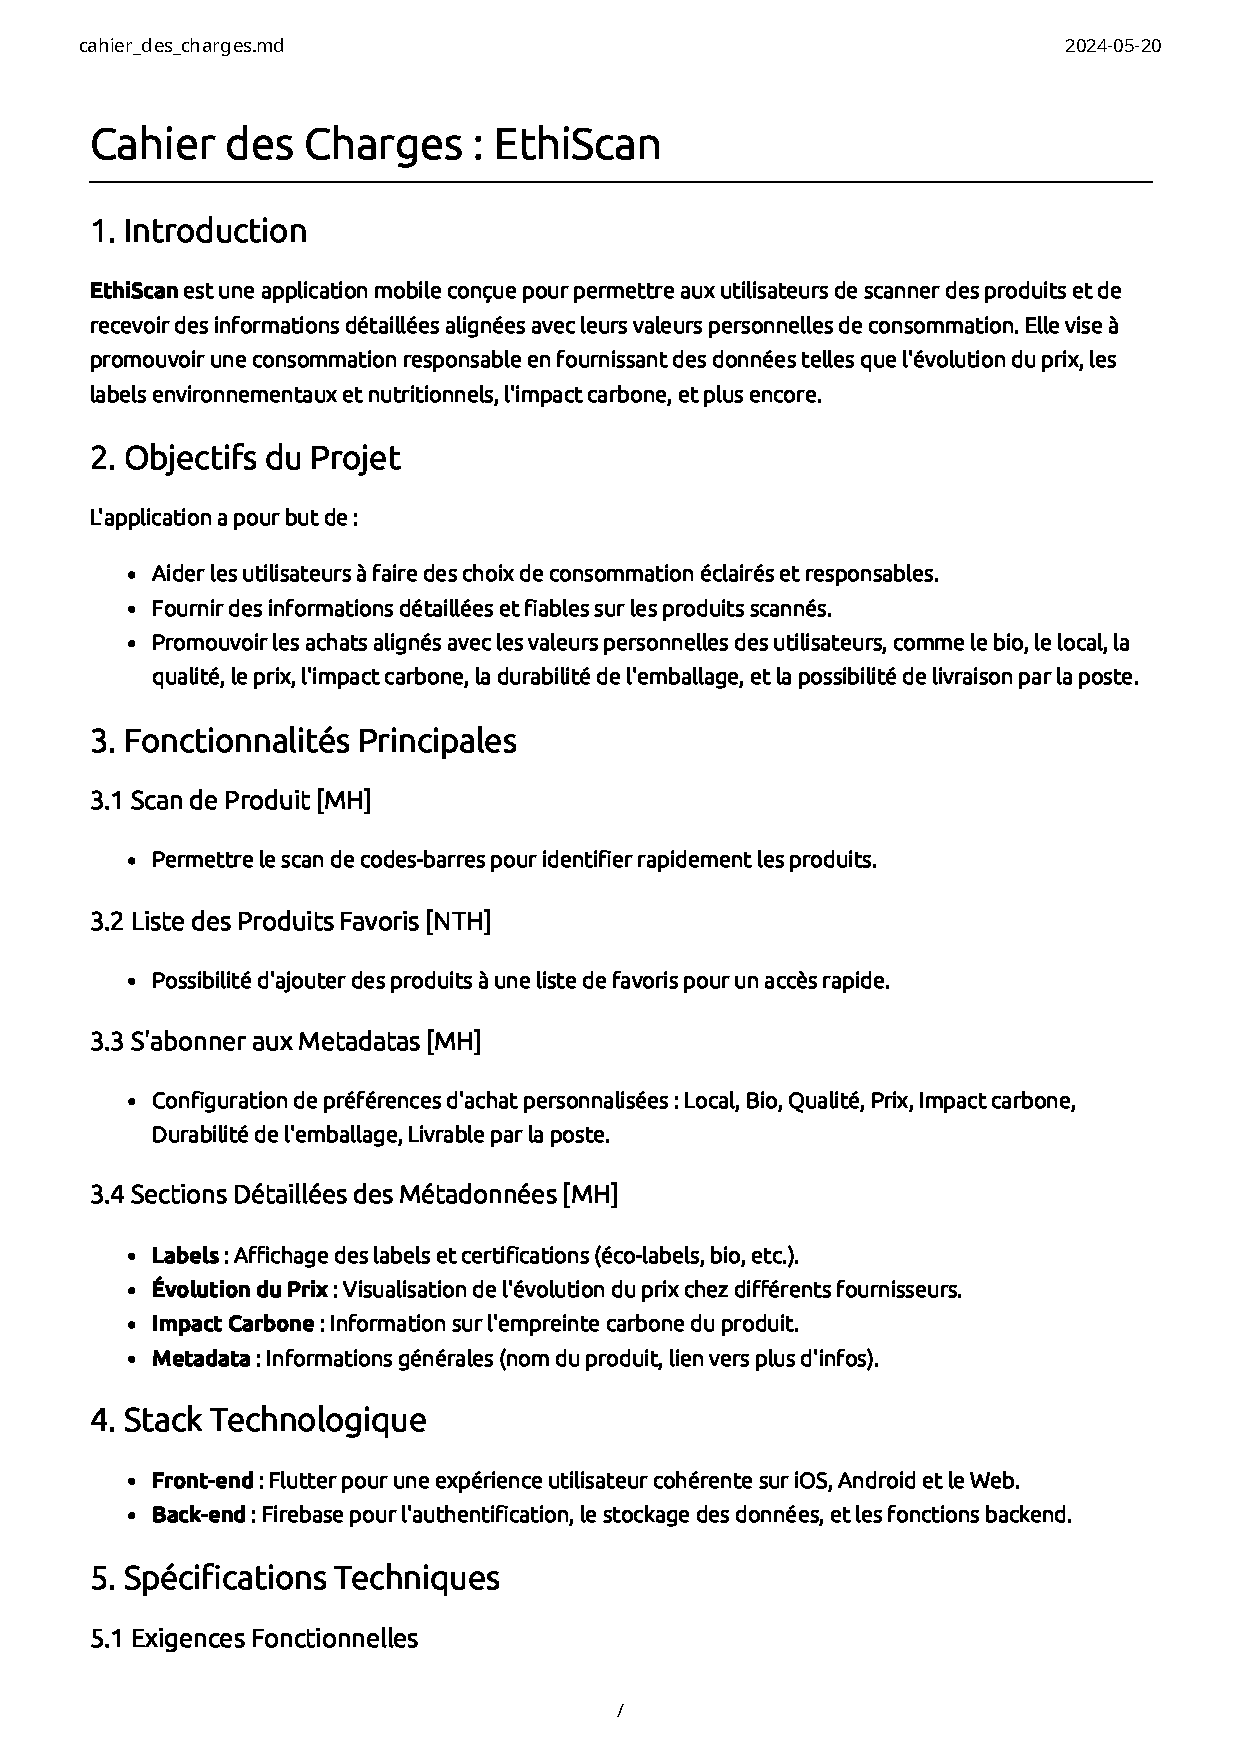
\includepdf[pages=-]{images/cahier_des_charges.pdf}